% !TEX root = ../../../../main/numb3rs_activities.tex
\newpage
\phantomsection
\addcontentsline{toc}{subsection}{107: Counterfeit Reality \label{ep107}}
\ep{107: Counterfeit Reality}
\setcounter{activity}{0}

Counterfeiters are producing small denomination bills by using the talent of an artist who they have kidnapped. Don and Charlie are afraid that the artist will be murdered as a liability by the criminals. The only way to find out the identity of the hostage is by running a match analysis between artistic pieces of several missing artists and the work seen in the counterfeit money. In order to do this Charlie uses Wavelet Analysis over the artists' work. We will explain below what Wavelet analysis is and how it is applied to image processing.

% Wavelet Analysis
\ltLarge{What is Wavelet Analysis?}


Wavelet analysis refers to the decomposition of finite energy signals into different frequency components by superposition of functions obtained after scaling and translating an initial function known as \textbf{Mother Wavelet}. Wavelet Analysis is different from other techniques in that it analyses frequency components with a resolution that matches their scale. 


In order to clarify the statement above we present an example of how Wavelet Analysis is used to analyze a discrete signal. Assume that you have a discrete signal given by a vector with 8 components,
	\begin{figure}[H]
	\centering
	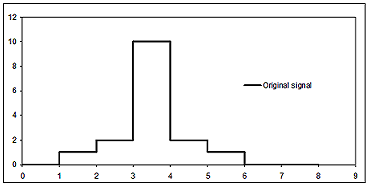
\includegraphics[width=0.75\textwidth]{../sections/seasons/season1/107/images/original_signal.png} \par
	$X= [ 0, 1, 2, 10, 2, 1, 0, 0 ]$
	\end{figure}


We show in the figure on the right a graphic representation of these data. Let's call $X(i)$ the $i$th component of the vector $X$ ($i=  0, 1, 2, \ldots, 7$). In the first step of the Wavelet decomposition of this signal we split our information into two vectors of 4 components, say $a(1), d(1)$. The $k$th component of $a(1)$ is equal to $\dfrac{X(2k) + X(2k+1)}{\sqrt{2}}$ and the $k$th component of $d(1)$ is equal to $\dfrac{X(2k) - X(2k+1)}{\sqrt{2}}$ ($k= 0, 1, 2, 3$). In our case, $a(1)= \left[ \frac{1}{\sqrt{2}}, \frac{12}{\sqrt{2}}, \frac{3}{\sqrt{2}}, 0 \right]$ and $d(1)= \left[ \frac{-1}{\sqrt{2}}, \frac{-8}{\sqrt{2}}, \frac{1}{\sqrt{2}}, 0 \right]$.


The vectors $a(1)$ and $d(1)$ are called the first level \textbf{approximation and detail coefficients} of the wavelet decomposition, respectively. On the right we show the graph of the first level approximation coefficients, which reveals that they represent the original signal in a different scale and explains why they are called \emph{approximation} coefficients.
	\begin{figure}[H]
	\centering
	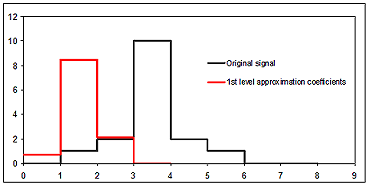
\includegraphics[width=0.75\textwidth]{../sections/seasons/season1/107/images/original_signal_2.png} 
	\end{figure}


In the next step we follow the exact same procedure over the vector $a(1)$ splitting it into two vectors of 2 components, $a(2)$ and $d(2)$, corresponding to the sums and differences of consecutive terms divided by $\sqrt{2}$, respectively. Then, $a(2)= \left[ \frac{13}{2}, \frac{3}{2} \right]$ and $d(2)= \left[ \frac{-11}{2}, \frac{3}{2} \right]$.


$a(2)$ and $d(2)$ are called the second level approximation and detail coefficients of the decomposition, respectively. Finally for the third and last step, we follow the same procedure over the vector $a(2)$, and we obtain two one-dimensional vectors $a(3)$ and $d(3)$ (the third level approximation and detail coefficients, respectively) where,  $a(3)= \frac{8}{\sqrt{2}}$ and $d(3)= \frac{5}{\sqrt{2}}$.


One of the nice features of the wavelet decomposition is that the reconstruction algorithm is very similar to the decomposition one. Let's assume that we have the approximation coefficient of the third level $a(3)$ and the decomposition coefficients corresponding to all the levels, $d(3)$, $d(2)$, $d(1)$. In order to get $a(2)$ from this information we take sums and differences of the components of $a(3)$ and $d(3)$ divided by $\sqrt{2}$. We obtain then,
	\[
	a(2)= \left[ \dfrac{\frac{8}{\sqrt{2}} + \frac{5}{\sqrt{2}}}{\sqrt{2}}= \dfrac{13}{2}, \dfrac{\frac{8}{\sqrt{2}} - \frac{5}{\sqrt{2}}}{\sqrt{2}} = \dfrac{3}{2} \right].
	\]
We proceed analogously with $a(2)$ and $d(2)$ in order to obtain the first level approximation coefficients,
	\[
	a(1)= \left[ \dfrac{\frac{13}{2} - \frac{11}{2}}{\sqrt{2}} = \dfrac{1}{\sqrt{2}}, \dfrac{\frac{13}{2} + \frac{11}{2}}{\sqrt{2}} = \dfrac{12}{\sqrt{2}}, \dfrac{\frac{3}{2}+\frac{3}{2}}{\sqrt{2}} = \dfrac{3}{\sqrt{2}},\dfrac{\frac{3}{2} - \frac{3}{2}}{\sqrt{2}} = 0 \right].
	\]
Finally, the same calculations over $a(1)$ and $d(1)$ reconstruct the original information,
	\[
	\hspace{-1.5cm} a(1)=\left[\frac{\frac{1}{\sqrt{2}}-\frac{1}{\sqrt{2}}}{\sqrt{2}}=0,\frac{\frac{1}{\sqrt{2}}+\frac{1}{\sqrt{2}}}{\sqrt{2}}=1,\frac{\frac{12}{\sqrt{2}}-\frac{8}{\sqrt{2}}}{\sqrt{2}}=2,\frac{\frac{12}{\sqrt{2}}+\frac{8}{\sqrt{2}}}{\sqrt{2}}=10,\frac{\frac{3}{\sqrt{2}}+\frac{1}{\sqrt{2}}}{\sqrt{2}}=2,\frac{\frac{3}{\sqrt{2}}-\frac{1}{\sqrt{2}}}{\sqrt{2}}=1,\frac{0+0}{\sqrt{2}}=0,\frac{0-0}{\sqrt{2}}=0 \right].
	\]
In order to understand the reasoning behind the calculations above it is convenient to see them from a ``continuous'' point of view. Let's call $h$ the function that takes the value 1 on the interval $[0,1)$ and 0 otherwise, and $g$ the function that takes the value 1 on $[0,0.5)$, $-1$ on $[0.5,1)$, and 0 otherwise. We can represent the signal $X$ as a combination of translations of the function $h$ as follows,
	\[
	0 \cdot h(t) + 1 \cdot h(t - 1) + 2 \cdot h(t - 2) + 10 \cdot h(t - 3) + 2 \cdot h(t - 4) + 1 \cdot h(t - 5) + 0 \cdot h(t - 6)+ 0 \cdot h(t - 7).
	\]
The key formulas behind the wavelet decomposition and reconstruction algorithms are the ones given by the representation of $h$ and $g$ as a combination of translations of versions of $h$ and $g$ in a different scale. More precisely,
	\[
	\begin{split}
	h(t)&= \frac{1}{\sqrt{2}} \left( \frac{1}{\sqrt{2}} \;h(2^{-1}t) \right)+ \frac{1}{\sqrt{2}} \left( \frac{1}{\sqrt{2}} \; g(2^{-1}t) \right) \\
	h(t-1)&= \frac{1}{\sqrt{2}} \left( \frac{1}{\sqrt{2}} \; h(2^{-1}t) \right) - \frac{1}{\sqrt{2}} \left( \frac{1}{\sqrt{2}} \; g(2^{-1}t) \right) \\
	\frac{1}{\sqrt{2}}\; h(2^{-1}t)&= \frac{1}{\sqrt{2}}\; h(t)+\frac{1}{\sqrt{2}} \; h(t-1) \\
	\frac{1}{\sqrt{2}} \; g(2^{-1}t)&= \frac{1}{\sqrt{2}} \; h(t)- \frac{1}{\sqrt{2}} \; h(t-1).
	\end{split}
	\]


We adopt the following notation,
	\[
	h_{i,k}=2^{i/2} \; h(2^it) \text{ and } g_{i,k}=2^{i/2}\; g(2^it) \text{ for }i,k \text{ integers}
	\]
Under this notation we observe, by using the formulas above, that the first level approximation and detail coefficients of the decomposition correspond to the coefficients in the decomposition of $X$ in terms of the scaled functions $h_{-1,k}$ and $g_{-1,k}$ as shown below,
	\[
	X= \frac{1}{\sqrt{2}}\; h_{-1,0} + \frac{12}{\sqrt{2}}\; h_{-1,1} + \frac{3}{\sqrt{2}}\; h_{-1,2} + 0 \; h_{-1,3} - \frac{1}{\sqrt{2}}\; g_{-1,0} - \frac{8}{\sqrt{2}}\; g_{-1,1} + \frac{1}{\sqrt{2}}\; g_{-1,2} + 0\; g_{-1,3}.
	\]
An analogous argument shows that the second level approximation and detail coefficients correspond to the coefficients in the decomposition of the signal generated by the first level approximation coefficients, in terms of translations of scaled versions of $h$ and $g$ given by 
	\[
	h_{-2,k} \text{ and } g_{-2,k} \text{ for } k \text{ an integer}.
	\]


In the \textbf{signal processing} terminology, we say that the functions above for i big analyze the small scales that correspond to the high frequencies of the signal (sudden changes in a short period of time) and the scaled functions for i small analyze the big scale features of the signal that correspond to the low frequencies, which give the signal its overall shape. This frequency analysis is local since each approximation and detail coefficient is calculated by using only part of the data and then it is adequate to study \textbf{non-stationary} signals (signals that do not repeat into infinity with the same periodicity).


\activity{\label{act:107_1}
Calculate the approximation and detail coefficients of the wavelet decomposition of the following signal:
	\[
	X= [ 1, 2, 10, 12, 5, 10, 11, 0 ]
	\]
Verify that the original signal can be recovered from your data by using the reconstruction algorithm described above.}

	\begin{figure}[H]
   	\centering
   	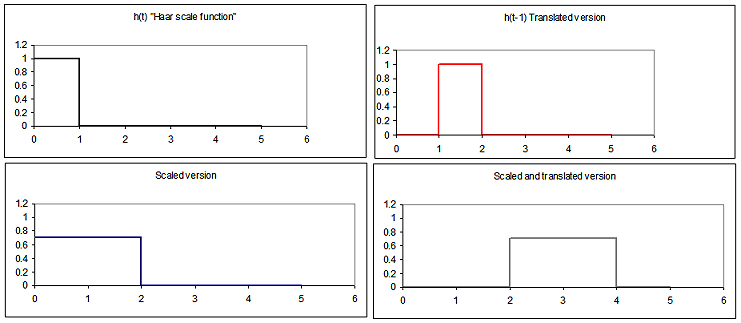
\includegraphics[width=\textwidth]{../sections/seasons/season1/107/images/haar.png} 
	\end{figure}

We mentioned above that wavelet analysis analyses frequency components with a resolution that matches their scale. In our case, the low frequencies are analyzed with the scaled versions of $h$ and $g$, and the main feature of these functions is that their support (i.e. the interval where they are not 0) get's larger as $i$ gets smaller (see figures above). This adaptive feature is what differentiates wavelet analysis from other techniques like \textbf{Fourier Analysis} where the functions used to analyze different frequencies have fixed support. The scheme presented in this example corresponds to what is called the \textbf{Haar Discrete Wavelet Transform}, which is closely related to the \textbf{Haar Multiresolution Analysis}; and the functions h and g are called the \textbf{Haar Scale and Mother Wavelet functions}, respectively. We refer the reader to \bref{``An introduction to wavelets''}{https://www.eecis.udel.edu/~amer/CISC651/IEEEwavelet.pdf} by Amara Graps and \bref{``A wavelet tour of signal processing''}{http://cas.ensmp.fr/~chaplais/Wavetour_presentation/Wavetour_presentation_US.html\#Chemins} by Stephane Mallat to find out more about Fourier Analysis, Multiresolution Analysis and Discrete Wavelet Transforms. We also recommend the introductory exposition of Yves Nievergelt in the book titled ``Wavelets Made Easy.'' Now we present an example that shows how wavelet analysis is used in data compression and explain how wavelet analysis is used to image processing.


\tangent{The Haar Scale function and Wavelet function are named after Alfred Haar, who proposed them as generators of bases for function spaces in 1902. The main disadvantage of these functions is that they are discontinuous and therefore not appropriate for the analysis of smooth signals. Only after 85 years, in 1987, \textbf{Ingrid Daubechies} discovered the first continuous wavelet functions with compact support and with her discovery Wavelet Analysis revolutionized the signal processing world. The Wavelet Transform constitutes a new method to decompose signals. This method represents a more adequate approach to lessen the restriction given by \textbf{Heisenberg's uncertainty principle}, which states that it is impossible to know the exact frequency and the exact time of occurrence of this frequency in a signal. This principle is explained in \hyperref[ep104]{Episode 104} as well.}


% Data Compression
\ltLarge{Data Compression and Image Processing}


Assume that after the wavelet decomposition described above we only keep the third level approximation coefficient and the first and second level detail coefficients, or equivalently we drop the value of $d(3)$. This represents a compression of data because we have to store only seven numbers instead of the initial eight. By assuming that $d(3)= 0$ and following the reconstruction algorithm as described above we obtain the new approximation coefficients and compressed signal given by
	\[
	\begin{split}
	\tilde{a}(2)&= [4, 4] \\
	\tilde{a}(1)&= \left[ \frac{-3}{2\sqrt{2}}, \frac{19}{2\sqrt{2}}, \frac{11}{2\sqrt{2}}, \frac{5}{2\sqrt{2}} \right] \\
	\tilde{X}&= \left[ \frac{-5}{4}, \frac{-1}{4}, \frac{3}{4}, \frac{35}{4}, \frac{13}{4}, \frac{9}{4}, \frac{5}{4},\frac{5}{4} \right]
	\end{split}
	\]

	\begin{figure}[H]
	\centering
	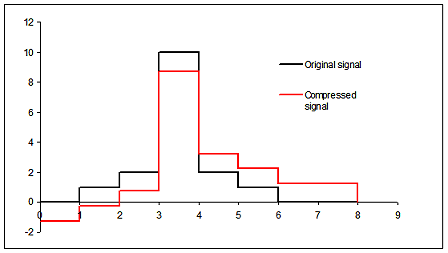
\includegraphics[width=0.75\textwidth]{../sections/seasons/season1/107/images/original_signal_3.png} 
	\end{figure}

We show below a graph that reveals some similarities between the original data and the compressed one. In general, data compression using wavelets consists in the storage of a restricted amount of detail coefficients of the wavelet decomposition. These coefficients, as their name suggest, contain the information about the details of the signal but are not important in order to recognize its ``big picture'' features.


% Image Processing
\ltLarge{Image Processing}


We can think of an image as a rectangular array of numbers, where each number represents the intensity at the corresponding pixel. The easiest way of generalizing the procedure explained before to the two dimensional case is by running the wavelet decomposition first over the rows of the image and then over its columns. Image compression again corresponds to the storage of the approximation coefficients and some of the detail coefficients. This procedure has been found to be very useful and has numerous applications. Perhaps the best-known application of wavelet analysis is used by the FBI, which, since 1993, uses a wavelet transform to compress digitalized fingerprint records (See the figure below).

	\begin{figure}[H]
	\centering
	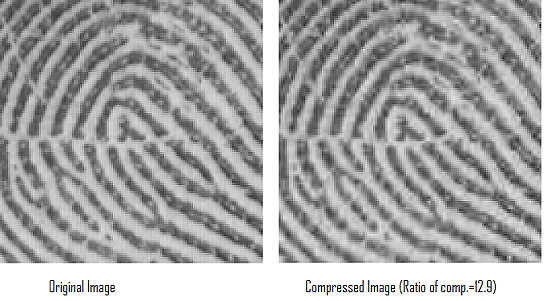
\includegraphics[width=0.5\textwidth]{../sections/seasons/season1/107/images/fingerprint.png} 
	\end{figure}

Image compression is not the only application of Wavelet Analysis. Since the analysis of the frequencies is done in a local manner there exist many applications of the wavelet transform to other image processing problems such as image restoration and edge detection. In edge detection edges of an image correspond to the occurrence of high frequencies in small portions of the signal, or equivalently to big detail coefficients in small scales. \bref{Matlab's wavelet toolbox}{http://www.mathworks.com/products/wavelet/?requestedDomain=www.mathworks.com} contains a comprehensive collection of routines to analyze data. All these nice features of the Wavelet transform helped Charlie to recognize similarities, in edges and scales of grey among others, between the artist's work and the one seen in the counterfeit money.


\activity{Find the compressed data obtained after dropping the third level detail coefficient of the wavelet decomposition of the signal given in \hyperref[act:107_1]{Activity I}, and draw a graph of your results.}